\documentclass[
  10pt,               % 120% Schriftgrösse
  oneside,            % einsitiger Druck
  a4paper,            % A4
  titlepage,          % inklusive Titelpage
  pointlessnumbers,	  % Kein Punkt hinter der Kapitelnummerierung
  halfparskip,        % Europäischer Satz mit abstand zwischen Absätzen
  pdftex,             % Direkt ins Pdf übersetzen, keine Kapitel
  liststotoc,         % Inhaltsverzeichnis inkl. Abbildungsverzeichnis
  bibtotoc]{scrreprt} % Inhaltsverzeichnis inkl. Literaturverzeichnis

%%%%%%%%%%%%%%%%%%%%%%%%%
% Allgemeine Packete    %
%%%%%%%%%%%%%%%%%%%%%%%%%

% Neue Rechtschreibung
\usepackage[german, ngerman]{babel}

% UTF 8
\usepackage[utf8]{inputenc}
\usepackage{units}
\usepackage{multirow}

% Ausgabefonts
\usepackage[T1]{fontenc}

% Euro Symbol (\texteuro}
\usepackage{textcomp}

% für die Gesamtseitenzahl
\usepackage{totpages}

% Paket für Farben
\usepackage{color}

% Bilder
%\usepackage{graphicx}

% Fliesstext um Bilder
\usepackage{wrapfig}

% Tabellen mit definierter Breite und zentriert
\usepackage{array}

\newcolumntype{x}[1]{%
>{\centering\hspace{0pt}}p{#1}}%

% Glossar alt
%\usepackage[style=super, header=none, border=none, number=none, cols=2, toc=true]{glossary}
%\makeglossary

% Glossar neu
%\usepackage{glossaries}
%\makeglossaries
%\printglossaries

% mehrere Befehle für die Tabellen
\usepackage{booktabs}

%Packet für absolut Positionierte Textboxen
\usepackage[absolute]{textpos} %showboxes zum besseren positionieren

% Packet für Boxen
%\usepackage{framed}

% Initialen
%\usepackage{lettrine}
%\DeclareFixedFont{\Yinit}{U}{yinit}{m}{n}{16}

% checkmarks
\usepackage{tikz}
\def\checkmark{\tikz\fill[scale=0.4](0,.35) -- (.25,0) -- (1,.7) -- (.25,.15) -- cycle;} 

%%%%%%%%%%%%%%%%%%%%%%%%%
% Seiteneinstellungen   %
%%%%%%%%%%%%%%%%%%%%%%%%%
\usepackage[
  portrait,
%   twoside,
  left=40mm,
  top=20mm,
  textwidth=145mm,
  textheight=252mm,
  %head=15mm,
  head=15mm,
  headsep=5mm,
  foot=8mm
]{geometry}

% Text muss nicht umbedingt bis zur Fusszeile reichen
\raggedbottom

%\usepackage[cam,axes,a3,center]{crop}
%\usepackage[frame,a4,center]{crop}

%%%%%%%%%%%%%%%%%%%%%%%%%
% Schriftart            %
%%%%%%%%%%%%%%%%%%%%%%%%%

%intent:
%USE: \-\hspace{2cm}

%\usepackage{courier}  % Courier für Code verwenden
%\usepackage{helvet}   % Helvetica
% Helvetic als Font verwenden
%\renewcommand{\familydefault}{\sfdefault}


%%%%%%%%%%%%%%%%%%%%%%%%%
% Mathematik Packete    %
%%%%%%%%%%%%%%%%%%%%%%%%%

% Verbesserte Mathematik Satz
\usepackage{amsmath}

% Zahlenmenngen in der Mathematik
\usepackage{amssymb}

% Times New Roman für Mathematik
\usepackage{mathptmx}


%%%%%%%%%%%%%%%%%%%%%%%%%
% Inhaltsverzeichnis    %
%%%%%%%%%%%%%%%%%%%%%%%%%
% Punkte im Inhaltsverzeichnis bei Sections
\usepackage{tocloft}
\renewcommand{\cftsecdotsep}{4.5}

%%%%%%%%%%%%%%%%%%%%%%%%%
% Literaturverzeichnis  %
%%%%%%%%%%%%%%%%%%%%%%%%%

%\usepackage[ngerman,ref]{backref}
%\renewcommand{\backrefpagesname}{Zitiert auf S.}
%renewcommand{\refname}{Quellenverzeichnis}

%%%%%%%%%%%%%%%%%%%%%%%%%
% Anhang			    %
%%%%%%%%%%%%%%%%%%%%%%%%%

\newcommand{\anhang}[1]{
	%\setsection{1}
    \setcounter{page}{1}
	\input{#1}
	\newpage
}

%%%%%%%%%%%%%%%%%%%%%%%%%
% Source Code Packete   %
%%%%%%%%%%%%%%%%%%%%%%%%%

% Codesegmente
\usepackage{listings}
\definecolor{darkblue}{rgb}{0,0,0.6}
\definecolor{darkred}{rgb}{0.6,0,0}
\definecolor{darkgreen}{rgb}{0,0.6,0}
\definecolor{red}{rgb}{0.98,0,0}
\lstloadlanguages{C,C++} % entsprechende Sprachen werden hier schon mal geladen, damit das Übersetzen schneller geht
\lstset{%
  language=C,
  basicstyle=\footnotesize\ttfamily,
  commentstyle=\itshape\color{darkgreen},
  keywordstyle=\bfseries\color{darkblue},
  stringstyle=\color{darkred},
  showspaces=false,
  columns=fixed,
  numbers=left,
  frame=none,
  numberstyle=\tiny,
  breaklines=true,
  showstringspaces=false,
  xleftmargin=1cm,
  tabsize=2
}%




%%%%%%%%%%%%%%%%%%%%%%%%%
% Makros                %
%%%%%%%%%%%%%%%%%%%%%%%%%

% Makros
\newcommand{\redbox}[1]
{\vspace*{2mm} \\ \fboxsep5mm \fboxrule0.5mm \fcolorbox{red}{white}{\parbox{1.5cm}{
\includegraphics[width=1cm]{Achtung.pdf}}\parbox{13cm}{\textcolor{black}{#1}
}}\vspace*{2mm}\\}

\newcommand{\redboxtitle}[2]
{\vspace*{2mm} \\ \textcolor{red}{\bfseries #1\smallskip} \\ \fboxsep5mm \fboxrule0.5mm \fcolorbox{red}{white}{\parbox{1.5cm}{
\includegraphics[width=1cm]{Achtung.pdf}}\parbox{13cm}{\textcolor{black}{#2}
}}\vspace*{2mm}\\}

% Fuer die Minipage um eine Tabelle und Abbildung nebeneinander Setzen
\makeatletter
\newcommand{\setcaptype}[1]{\renewcommand{\@captype}{#1}}
\makeatother


%%%%%%%%%%%%%%%%%%%%%%%%%
% Kopf und Fusszeile    %
%%%%%%%%%%%%%%%%%%%%%%%%%
% 7. Kopf und Fusszeilen
\usepackage{totpages}               % Paket für die Gesamtseitenzahl
\usepackage{scrpage2}
\pagestyle{scrheadings}
\renewcommand*{\chapterpagestyle}{scrheadings}
\clearscrheadfoot
%\setkomafont{pagefoot}{\normalfont\sffamily}
\automark[]{chapter}
%\ihead{NTB-Robotersteuerung}
\ihead{VT1: EEROS Sequencer}
\ohead{\headmark}
\setheadsepline{0.5pt}[\color{HeadBlue}] 
%\ifoot{Benno Jung • Michael Krähenbühl • Martin Züger}
\cfoot{- \thepage{} -}
%\setfootsepline{0.5pt}
%%Kopf- und Fusszeile
\definecolor{HeadBlue}{rgb}{0,0.41,0.71}
\definecolor{FootBlack}{rgb}{0,0,0}
\addtokomafont{pagehead}{\color{HeadBlue}} 
\addtokomafont{pagefoot}{\color{FootBlack}}
%\usepackage{eso-pic}
%\usepackage{scrpage2}
%\usepackage{extramarks}
\usepackage[final]{pdfpages}
%%\pagestyle{scrheadings}
%%\clearscrheadfoot
%% Schriftart auf die Normale Schrift setzen
%%\setkomafont{pagefoot}{\normalfont\sffamily}
%%\automark[]{section} % \leftmark zeigt die aktuelle Section an, \rightmark bleibt leer
%
%%Kopfzeile
%%\ihead{NTB}
%%\ohead{\leftmark}
%%\lehead{\hspace*{1cm}\begin{large}\leftmark\end{large} \AddToShipoutPicture*{%
%%  \AtPageUpperLeft{\put(0,\LenToUnit{-9.4mm}){%
%%    \colorbox{HeadBlue}{\parbox[t][6mm]{1.8cm}{\ }}%
%%    \colorbox{black}{\parbox[t][6mm]{0.1cm}{\ }}}}}}
%%\rohead{\begin{large}\leftmark\end{large}\hspace*{1cm} \AddToShipoutPicture*{%
%%  \AtPageUpperLeft{\put(\LenToUnit{\paperwidth},\LenToUnit{-9.4mm}){\kern-2.3cm%
%%    \colorbox{black}{\parbox[t][6mm]{0.1cm}{\ }}%
%%    \colorbox{HeadBlue}{\parbox[t][6mm]{1.8cm}{\ }}}}}}
%%\rehead{\begin{large}NTB\end{large}}
%%\lohead{\begin{large}NTB\end{large}}
%%\setheadsepline{1.2pt}
%\usepackage{ifthen}
%\newboolean{SectionOnPage}
%\renewcommand{\sectionmark}[1]{\setboolean{SectionOnPage}{true}\markboth{#1}{#1}}
%\newcommand{\headerblackbox}{\colorbox{black}{\parbox[c][6mm]{0.1cm}{\ }}}
%\newcommand{\headerbluebox}[1]{\colorbox{HeadBlue}{\parbox[c][6mm]{1.8cm}{%
%%       \ifnum\value{section}>0
%%         \ifthenelse{true}{H}{#1\textbf{\begin{large}\color{white}{\sffamily{\arabic{section}}}\end{large}}}
%%       \else
%          #1 \textbf{\begin{large}\color{white}{\sffamily{\ }}\end{large}}
%%       \fi
%}}}
%\newcommand{\headerbluetext}[1]{\textbf{\begin{large}\color{HeadBlue}{#1}\end{large}}}
%%\newcommand{\headerNTB}{\headerbluetext{NTB}}
%\newcommand{\headerNTB}{\includegraphics[height=1.2cm]{ntb}}
%\newcommand{\headerleftmark}{\headerbluetext{\firstleftmark}}
%
%\lehead{\hspace*{5mm}\headerleftmark \AddToShipoutPicture*{%
%  \AtPageUpperLeft{\put(0,\LenToUnit{-13.4mm})}}}
%
%\rohead{\headerleftmark \hspace*{5mm} \AddToShipoutPicture*{%
%  \AtPageUpperLeft{\put(\LenToUnit{\paperwidth},\LenToUnit{-13.4mm})}}}
%
%
%%\rehead{\headerNTB}
%%\lohead{\headerNTB}
%\rehead{Seite \thepage{}}
%\setheadsepline{0.8pt}
%\renewcommand*{\chapterpagestyle}{scrheadings}
%%\setheadsepline{0.5pt}[\color{blue}]
%
%%Fusszeile
%%\ifoot{Marcel Gehrig, Egemen Yesil}
%%\cfoot{\today}
%\cfoot{- \thepage{} -}
%%\ofoot{\thepage{} / \ref{TotPages}}
%%\setfootsepline{0.5pt}

%%%%%%%%%%%%%%%%%%%%%%%%%
% Informationen         %
% über den Autor        %
%%%%%%%%%%%%%%%%%%%%%%%%%

\title{VT1: EEROS Sequencer 2017}
\author{Marcel Gehrig}
\date{Januar 2017}


%%%%%%%%%%%%%%%%%%%%%%%%%
% Pdf Einstellungen     %
%%%%%%%%%%%%%%%%%%%%%%%%%

% Paket für Links innerhalb des PDF Dokuments und Pdf Informationen
\definecolor{LinkColor}{rgb}{0,0,0}
\usepackage[
  pdftitle={VT1 EEROS Sequencer},
  pdfauthor={Marcel Gehrig},
  pdfcreator={Texmaker},
%  pdfsubject={VT1 EEROS Sequencer},
  pdfsubject=pdftitle,
  pdfkeywords={Schlussbericht,Vertiefungsarbeit,EEROS,Sequencer,C++,Roboter Steuerung}]{hyperref}
\hypersetup{colorlinks=true,
  linkcolor=LinkColor,
  citecolor=LinkColor,
  filecolor=LinkColor,
  menucolor=LinkColor,
  urlcolor=LinkColor}

% Packet um Dateien in das PDF einzubetten
\usepackage{attachfile}
\usepackage{pdfpages}
%%%%%%%%%%%%%%%%%%%%%%%%%
% Farben                %
%%%%%%%%%%%%%%%%%%%%%%%%%

\definecolor{Blue}{rgb}{0,0,1}
\definecolor{Red}{rgb}{1,0,0}
\definecolor{Green}{rgb}{0,1,0}

%%%%%%%%%%%%%%%%%%%%%%%%%%%
%%%%%%%%%%%%%%%%%%%%%%%%%%%
%% ACHTUNG:              %%
%% Informationen über    %%
%% den Autor müssen in   %%
%% folgenden Abschnitten %%
%% angepasst werden:     %%
%%                       %%
%% - PDF EINSTELLUNGEN   %%
%% - KOPF UND FUSSZEILE  %%
%% - AUTOR               %%
%%%%%%%%%%%%%%%%%%%%%%%%%%%

%Tiefe der nummerierten Ebene
\setcounter{tocdepth}{4} %Anzeigetiefe im Inhaltsverzeichniss
\setcounter{secnumdepth}{4} %Nummerierungstiefe
\renewcommand*{\chapterpagestyle}{scrheadings} %Kopfzeile auch bei \chapter
\renewcommand*{\chapterheadstartvskip}{\vspace*{-\topskip}}  %Abstand korrigieren von Kopfzeile zu \chapter
\setlength{\cftbeforetoctitleskip}{-2mm} 
\setlength{\cftaftertoctitleskip}{0.5mm}
\usepackage{placeins} %um floatbarrier zu benutzen
%\usepackage{mathtext}

%Pfad für die Bilder Festlegen
%\graphicspath{{Bilder/},{Icons/},{Logo/},{Template/},{Ismages/},{}}
\graphicspath{{images_P/},{}}
%%Grosser Zeilenabstand für Korrektur
% \usepackage{setspace}
% \linespread{2}

%%%%%%%%%%%%%%%%%%%%%%%%%
% Dokument              %
%%%%%%%%%%%%%%%%%%%%%%%%%
\begin{document}
	\renewcommand{\thepage}{\roman{page}}
	\renewcommand{\bibname}{Quellenverzeichnis}
%	
\begin{titlepage}
	\setlength{\TPHorizModule}{\paperwidth}
	\setlength{\TPVertModule}{\paperheight}
	
	
	
	\begin{textblock}{0.95}[0.4,-0.5](0.5,0.04)
	\makebox{
\includegraphics[width=5.5cm]{images/eeros_logo.png}}
	\end{textblock}
	\begin{textblock}{0.3}[0.1,-0.5](0.68,0.03)
	\makebox{
\includegraphics[width=5.5cm]{images/ntb_logo.jpg}}
	\end{textblock}
    \vspace*{6cm}
    \begin{center}
    	\Huge{\color{HeadBlue}{Eine ROS Anbindung für EEROS\\}}
		\vspace*{5cm}
		\normalsize
      	{\color{HeadBlue}{\sffamily{
      		\textbf{Vertiefungsarbeit 2 1017} \\
      		\vspace*{1cm}
      		von \\
      		\vspace*{1cm}
%			~\newline
      		\textbf{Marcel Gehrig}
      		}}}\\
		\vspace*{2cm}      	
%		\includegraphics[height=4cm]{images/logo_valens}


    \vspace*{3cm}
    \color{HeadBlue}
    \begin{tabular}{p{4cm}l}
      Advisor: & Dr. Urs Graf \\
      Abgabedatum: & 25. August 2017
    \end{tabular}\\
    \end{center}
  \end{titlepage}




%	\newpage
%	
\chapter*{Kurzfassung}
In dieser Arbeit wird vorgestellt, wie eine EEROS Applikation in einem ROS Netzwerk eingebunden werden kann und wie bestehende ROS Werkzeuge genutzt werden können, um EEROS Applikationen zu erweitern.

EEROS ist ein Roboter-Framework, das an der NTB entwickelt wird.
Es konzentriert sich aber im Gegensatz zu ROS nicht darauf, mehrere Komponenten von einem Roboter-System in einem Netzwerk zu verbinden sondern die grosse Stärke von EEROS ist die Echtzeitfähigkeit.
In EEROS können komplexe Kinematiken abgebildet und in Echtzeit geregelt werden.
Da ROS nicht echtzeitfähig ist, können Regler in ROS nicht gerechnet werden.
EEROS schliesst diese Lücke.

ROS, oder Robot Operating System, ist ein Set von Softwarebibliotheken und Werkzeugen um Roboteranwendungen zu schreiben.
Ein ROS Netzwerk besteht aus diversen Knoten.
Jeder Knoten kann einen Sensor, einen Aktor, einen Datenverarbeitungsknoten oder eine Simulation (Gazebo) darstellen.
Es besteht aus dem Kern und mehreren Packages, die das Framework erweitern können.
Die Packages sind oft frei erhältlich und erlauben es, diverse Hardware mit einem standardisierten Protokoll ansprechen zu können.
Eine grosse Community entwickelt nicht nur den Kern von ROS immer weiter, sondern veröffentlicht auch immer neue Packages um die Funktionalität von ROS zu erweitern.

In dieser Arbeit wird EEROS erweitert, damit zukünftige EEROS Applikationen mühelos in ein ROS Netzwerk eingebunden werden können.
Dabei wurde speziell darauf geachtet, dass EEROS Applikationen auch mit Gazebo Simulationen verbunden werden können, um die Applikation oder Regelung testen zu können.
Mit den, in dieser Arbeit entwickelten Erweiterungen können EEROS Applikationen zukünftig Daten von ROS-Knoten lesen, Daten an ROS-Knoten schicken und mit einer Gazbeo Simulation können EEROS Applikationen getestet werden, ohne dass die Hardware des Roboters vorhanden sein muss.
Zusätzlich kann das ROS Netzwerk und ROS Werkzeuge neu auch genutzt werden, um lückenlos Daten von EEROS Signalen aufzuzeichnen und zu visualisieren.



%The Robot Operating System (ROS) is a set of software libraries and tools that help you build robot applications. From drivers to state-of-the-art algorithms, and with powerful developer tools, ROS has what you need for your next robotics project. And it's all open source.



%Im Auftrag des Industriepartner Variosystems wurde ein kostengünstiger, auf dem BeagleBone Black basierter Platinencomputer entwickelt. Der BeagleBone Black, im weiteren Text als BBB bezeichnet, ist ein vollständiger Computer für Linux-basierte Betriebssysteme. Standardmässig wird es mit dem Betriebssystem Debian ausgeliefert, welches für diese BA ebenfalls benutzt wird. Im Verlauf dieser Arbeit wurden insgesamt 5 Exemplare hergestellt, die alle bei Variosystems bestückt wurden. Mit einem Cape, einer aufsteckbaren Platine für den BBB, wurde der Computer mit WLAN, Bluetooth Low-Energy, GSM/GPRS und einem Touchscreen ergänzt. Dieses Cape ist nicht nur mit dem von uns gebauten BBB-Derivat kompatibel, sondern auch mit dem kommerziell erhältlichen, originalen BBB. Die Kombination des BBB mit dem Cape wird im Folgenden Communication-Bone, oder kurz ComBone genant. Der Name ist eine Wortkombination des englischen Wortes "Communication" \ für die Kommunikationsfähigkeit des Capes über verschiedene Kanäle, sowie dem Wort "Bone", welches bereits im Namen des originalen BBB genutzt wird.
%
%Bei der Entwicklung der Hard- und Software ist darauf geachtet worden, dass die einzelnen Funktionen möglichst modular sind. Wenn bestimmte Funktionen nicht benötigt werden, wie zum Beispiel der HDMI Anschluss des BBB oder die WLAN-Funktion des Capes, können die entsprechenden Bauteile bei der Produktion einfach nicht bestückt werden. Dies kann, besonders bei grösseren Stückzahlen, viel Geld sparen. Des Weiteren können auch einige Module, beziehungsweise Funktionen, einfach kopiert und in anderen Projekten verwendet werden.
%
%Ein möglicher Einsatzbereich dieses Computers mit dem Cape ist die Verbindung von einem Gerät, wie etwa ein Sensor oder ein abgelegener Stromgenerator, mit dem Internet. Der ComBone kann sich mit einer LAN-Verbindung, mit WLAN oder über das mobile GSM Netz, wie es auch ein Mobiltelefon verwendet, ins Internet einwählen. Dies macht den ComBone zu einem  hochflexibles Gerät, welches diverse Einsatzmöglichkeiten hat.





%\section*{Abstract}
%TODO Englischübersetzung

	\newpage
	\makeatletter
	\addtocontents{toc}{\protect\thispagestyle{scrheadings}}
	\renewcommand{\tableofcontents}{\section*{\contentsname} \pagestyle{scrheadings} \@starttoc{toc}}
	\makeatother
	\tableofcontents
	\newpage
	\renewcommand{\thepage}{\arabic{page}}
	\setcounter{page}{1}
	
%	\chapter{Einleitung}


\section{Repositories}
Für diese Arbeit werden folgende Git-Repositories verwendet.
Alle Repositories werden auf GitHub gehostet.

Das Haupt-Repository enthält alle digitalen Daten von dieser Arbeit inklusive aller anderen Sub-Repositories (Submodule).
Mit folgendem Befehl können alle Repositories auf einmal geklont werden:

\textit{git clone --recursive -j8 https://github.com/MarcelGehrig2/VT2.git}

\begin{tabular}
  { l						l			 												l						}

% Name						URL   														Branch     			
  \textbf{Name}				& \textbf{URL}												& \textbf{Branch}		\\
  VT2						& https://github.com/MarcelGehrig2/VT2.git					& master				\\
  EEROS						& https://github.com/MarcelGehrig/eeros-framework			& ROSVt2				\\
  EEROSTestApp				& https://github.com/MarcelGehrig2/testAppEEROSEVT2.git		& master		 		\\
  SimpleROSNode				& https://github.com/MarcelGehrig2/simpleROSNodeVt2.git		& master				\\
  Bericht					& https://github.com/MarcelGehrig2/berichtVt2.git			& master				\\
\end{tabular}

	\chapter{Feature List}
\label{chapter:featureList}
\section{Einleitung}
In diesem Kapitel werden \textit{Features} beschrieben, die im Rahmen dieser Arbeit implementiert werden sollen.
Für alle \textit{Features} wird der Nutzen beschrieben und auch mögliche Probleme identifiziert.
Die \textit{Features} werden in Teilziele unterteilt und nach Nutzen und geschätztem Arbeitsaufwand bewertet.
Am Schluss werden alle Teilziele nach dem besten Nutzen-Aufwand-Verhältnis sortiert, um die die \textit{Features} zu identifizieren, welche sich am meisten zu implementieren lohnen.


\section{Essential Features}
\subsection{Beschreibung}
\textit{Essential Features} sind alle Features, welche von allen anderen Features benötigt werden und grundsätzlich notwendig sind, um EEROS mit ROS zu verwenden.
Diese Features sind notwendig, dass eine EEROS-Applikation überhaupt als unabhängiger ROS-Knoten funktionieren kann.


\section{Daten über einen ROS-Knoten empfangen}
\subsection{Beschreibung}
Eine EEROS-Applikation soll Daten von diversen Quellen über einen ROS-Knoten empfangen können.
Mögliche Quellen sind Sensoren (Microsoft Kinect) oder Steuerungsbefehle.
Die Steuerungsbefehle sollen über eine GUI, eine Tastatur oder einen XBox-Controller\footnote{siehe dazu 'joy'\_packet http://wiki.ros.org/joy} gesendet werden können.


\section{Logging (Protokollierung)}
\subsection{Beschreibung}
Mit \textit{Logging} sind Ausgaben gemeint, die den aktuellen Status der EEROS-Applikation wiedergeben.
Sie können auch für Fehlermeldungen und Debug-Informationen verwendet werden.

Das EEROS-Framework hat bereits eine Logger-Funktionalität.
In der aktuellen EEROS-Version kann der \textit{Loggers}  mit folgenden Zeilen benutzt werden\footnote{http://wiki.eeros.org/tools/logger/start?s[]=log}:
\lstset{language=C++}
\begin{lstlisting}
StreamLogWriter w(std::cout); Logger log(); log.set(w);
log.info() << "Logger Test";
int a = 298;
logg.warn() << "a = " << a;
log.error() << "first line" << endl << "second line"; 
\end{lstlisting}

In EEROS erfolgt die Ausgabe des \textit{Loggers} über die Konsole (\textit{StreamLogWriter}) oder in eine Datei (\textit{SysLogWriter}).
Wenn die Ausgabe auf einem anderen PC erfolgen soll, z.B. bei einem ferngesteuerten Roboter, kann eine SSH-Verbindung hergestellt werden.

EEROS bietet auch eine Möglichkeit um Informationen im \textit{Control System} zu loggen\footnote{http://wiki.eeros.org/tools/logger\_cs/start}.
Dabei stellt sich das Problem, dass das \textit{Control System} normalerweise sehr oft (1000 mal in der Sekunde) ausgeführt wird und den Bildschirm mit Informationen überfluten würde.
Es existiert aber bereits eine Lösung mit \textit{Periodic Functions}, damit die Daten mit einer viel kleineren Frequenz ausgegeben werden.
Die Lösung mit den \textit{Periodic Functions} ist aber nicht intuitiv und wird oft, besonders in der Debugging-Phase nicht genutzt und umgangen.

ROS hat mit der \textit{ROS console}\footnote{http://wiki.ros.org/rosconsole} eine ausgereifte Logging-Funktion integriert.
Mit der \textit{Throttle-Funktion} \texttt{ROS\_DEBUG\_THROTTLE(period, ...)} bietet ROS eine sehr bequeme Möglichkeit, um eine Information nur einmal in einem bestimmten Zeitraum auszugeben.
Weitere Funktionen sind noch:

\begin{itemize}
\item ROS\_DEBUG\_COND(cond, ...)
\item ROS\_DEBUG\_ONCE(...)
\item ROS\_DEBUG\_DELAYED\_THROTTLE(period, ...)
\item ROS\_DEBUG\_FILTER(filter, ...)
\end{itemize}

Wie auch EEROS hat ROS verschiedene \textit{verbosity levels} um Debug-Informationen von normalen Informationen, Warnungen und Fehlern zu unterscheiden.

Ein weiterer Vorteil bei ROS ist, dass die Ausgaben irgendwo im ROS-Netzwerk, also auch auf einem anderen PC, gelesen und in eine Datei gespeichert werden können.
Zusätzlich existieren schon ausgereifte Programme, welche die Ausgaben live filtern, farblich hervorheben und ausgeben können.
\textit{rqt\_console} ist ein solches Programm, das auch schon standardmässig mit ROS installiert wird.
In Bild \ref{fig:rqtConsole} ist ein Screenshot von \textit{rqt\_console} zu sehen.

\begin{figure}[!ht]
\centering
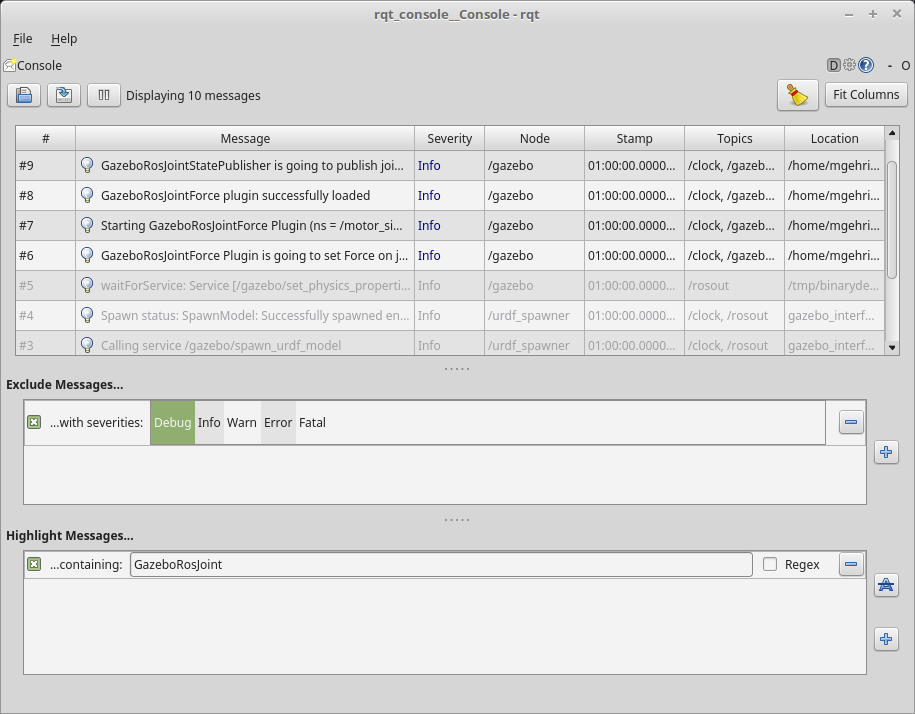
\includegraphics[angle=0,width=\textwidth]{images/screenshotRqtConsole.png}
\caption{\textit{rqt\_console} ist ein ROS-Tool, um Log-Nachrichten darzustellen und zu filtern}
\label{fig:rqtConsole}
\end{figure}


\section{Anzeige von Prozessvariablen}
\subsection{Beschreibung}
Prozessvariablen sind, im Gegensatz zu den Log-Ausgaben, einzelne Zahlen oder Datenpunkte, wie beispielsweise die Position eines Encoders.
Die Variablen können in einem GUI angezeigt werden.
Im einfachsten Fall zeigt das GUI die Variablen in einer einfachen Konsole an.
In vielen Fällen ist es aber von Vorteil, wenn eine oder mehrere Variablen in einem Graphen visualisiert werden können.

\subsection{Zu erwartende Probleme}
Bei Prozessvariablen gilt es zu beachten, dass sehr schnell eine grosse Menge von Daten anfallen können.
Dabei ist nicht nur die Bandbreite ein Problem, sondern auch die Latenz.
Im konkreten Fall bedeutet dies, dass in einem \textit{Control System} bei jedem Durchlauf innerhalb sehr kurzer Zeit (typischerweise \unit[1]{msec}) neue Daten produziert werden.
Wenn das ROS-Netzwerk nicht innerhalb einer Millisekunde die Daten wegschicken kann, kann es sein, dass Daten verloren gehen.

Eine Lösung für die zu geringe Latenz des ROS-Netzwerks wäre ein Buffer, der den hochfrequenten Datenstrom abfängt und in längeren Zeitabständen (etwa \unit[0.1]{s} bis \unit[1]{s}) Datenpakete mit den Daten schickt.

%TODO auf performance messungen verweisen dei zeigen, dass das kein problem is

Wenn aber die Bandbreite zu hoch ist, das heisst, wenn mehr Daten durch das ROS-Netzwerk geschickt werden, als das Netzwerk übertragen kann, dann reicht ein einfacher Buffer nicht mehr aus.
Folgende Techniken könnten das Problem lösen:
\begin{itemize}
\item \textbf{Throttle:} Funktioniert wie der Logger mit \textit{Throttle}-Funktionalität. Die meisten Daten werden verworfen und nur jeder x-te Wert wird geschickt.
\item \textbf{Zeitbegrenzter Buffer:} Ein Buffer speichert über eine begrenzte Zeit die Daten und schickt sie dann mit reduzierter Bandbreite über das Netzwerk.
\item \textbf{Filter:} Es werden nur Daten gesendet, die eine bestimmte Bedingung erfüllen, wenn beispielsweise deren Wert grösser als 10 ist.
\item \textbf{Statistik:} Für eine gewisse Anzahl von Datenpunkten werden statistische Werte, wie z.B. Mittelwert, Minimum und Maximum berechnet. Dem Netzwerk werden nur die berechneten Werte gesendet.
\end{itemize}


\section{Simulation mit Gazebo}
\subsection{Beschreibung}
\textit{Gazebo} ist eine Simulationssoftware für Roboter.
Wenn der physikalische Roboter von \textit{Gazebo} simuliert wird, dann kann die EEROS-Applikation getestet werden, ohne dass die Hardware vorhanden sein muss.
Nachdem die Applikation und die Regelung mit der Simulation getestet und verfeinert wurden, kann sie auf dem richtigen Roboter getestet werden.

Idealerweise wird dafür die HAL von EEROS genutzt.
So muss nur die Konfigurationsdatei der HAL angepasst werden, wenn von der Simulation zur richtigen Hardware gewechselt wird.

\subsection{Zu erwartende Probleme}
Eine Simulation muss nicht in Echtzeit erfolgen.
Wenn es eine komplexere Simulation ist, oder wenn die Simulation visualisiert werden soll, dann ist der Rechner oft zu langsam, um die Simulation in Echtzeit zu rechnen.
Die Kommunikation mit ROS ist ebenfalls nicht echtzeitfähig.

Eine Simulation von einem dynamischen System ist aber stark abhängig von der Zeit.
Es muss also sichergestellt werden, dass die Simulation und auch die EEROS-Applikation mit der richtigen Zeit rechnet, damit auch Regler getestet werden können.
Zusätzlich muss sichergestellt werden, dass die Simulation und die Applikation abwechselnd rechnen, um \textit{Race Conditions} zu vermeiden.


\section{Bewertung der verschiedenen Features und Teilziele}
\subsection{Beschreibung des Punktesystems}
In Tabelle \ref{Bewertungstabelle} werden alle oben genannten Features in Teilziele aufgeteilt und deren Nutzen und Aufwand mit einem Wert zwischen 0 und 10 bewertet.
Die Punkte für jedes Teilziel werden berechnet, indem der Nutzen durch den Aufwand dividiert wird.
Mit dieser Methode sollen diejenigen Teilziele gefunden werden, die mit möglichst kleinem Aufwand einen möglichst grossen Nutzen bringen.

In der Tabelle \ref{BewertungstabelleSortiert} sind alle Teilziele nach dem Punktewert sortiert.
Nur die \textit{Essential Features} bilden eine Ausnahme, da sie von allen anderen Features benötigt werden.
Deshalb sind sie an erster Stelle.

Alle Features werden dann der Reihe nach implementiert.
Sollte im Rahmen dieser Arbeit nicht genügend Zeit vorhanden sein, um alle Teilziele zu implementieren, dann werden die Teilziele ganz unten, also die mit dem schlechtesten Nutzen-Aufwand-Verhältnis, nicht implementiert.


\subsection{Bewertungstabelle}
\label{Bewertungstabelle}
\begin{tabular}
  { l								| l			 								l			 l			 l }
  \textbf{Feature}					& \textbf{Teilziel}	& \textbf{Nutzen}	& \textbf{Aufwand}	& \textbf{Punkte}	\\ \hline
  
% Feature							  Teilziel   								Nutzen      Aufwand     Punkte
  Essential							& 1. Unabhängiger ROS-Knoten				& 10		& 3			& 3.3		\\
  									& 2. CMAKE									& 10		& 4			& 2.5		\\ \hline
  Daten empfangen					& 1. Einfacher ROS-Knoten					& 8			& 3			& 2.7		\\
  									& 2. Generischer ROS-Knoten					& 8			& 4			& 2.0		\\
  									& 3. HAL									& 8			& 7			& 1.1		\\
  									& 4. Generischer Tastaturknoten				& 7			& 5			& 1.4		\\ 
  									& 4. XBox-Controller						& 7			& 5			& 1.4		\\ \hline
  Daten senden						& 1. Konsolenausgabe 						& 8			& 5			& 1.6		\\
  									& 2. Diagramm								& 8			& 6			& 1.3		\\
  									& 3. Gazebo									& 10		& 8			& 1.3		\\
  									& 4. Throttle-Funktion						& 8			& 6			& 1.3		\\
  									& 5. Zeitbegrenzter Buffer					& 6			& 6			& 1.0		\\
  									& 6. Filter									& 6			& 6			& 1.0		\\
  									& 7. Statistik								& 7			& 7			& 1.0		\\ \hline
  Logging 							& 1. EEROS-Logger umlenken					& 4			& 4			& 1.0		\\
  									& 2. \textit{Verbosity levels} beibehalten	& 2			& 5			& 0.4		\\
  									& 3. \textit{Throttle}-Funktionalität		& 4			& 6			& 0.7		\\
  									& 4. \textit{Conditional}-Funktionalität 	& 3			& 3			& 1.0		\\
  									& 5. \textit{Once}-Funktionalität			& 3			& 3			& 1.0		\\
  									& 6. \textit{Filter}-Funktionalität			& 1			& 3			& 0.3		\\
  									& 7. \textit{Delayed-Throttle}-Funkt.		& 1			& 3			& 0.3		\\ \hline
%  Manipulieren von Prozessvar.		& 1. Ausgänge setzen						& 8			& 4			& 2.0		\\
%  									& 2. Konstanten setzen						& 6			& 4			& 1.5		\\ \hline
  Simulation mit Gazebo				& 1. Einfacher PI Regler					& 8			& 5			& 1.6		\\
  									& 2. Korrekter Zeitstempel und Sync.		& 9			& 6			& 1.5		\\ \hline
\end{tabular}

\subsection{Bewertungstabelle sortiert}
\label{BewertungstabelleSortiert}
\begin{tabular}
  { l								| l			 								l			 l			 l 		l}
  \textbf{Feature}					& \textbf{Teilziel}	& \textbf{Nutzen}	& \textbf{Aufwand}	& \textbf{Punkte}	& \textbf{Impl.}	\\ \hline
  
% Feature							  Teilziel   							Nutzen      Aufwand     Punkte
  Essential							& Unabhängiger ROS-Knoten				& 10		& 3			& 3.3	&\cmark	\\
  Essential							& CMAKE									& 10		& 4			& 2.5	&\cmark	\\ 
  Daten empfangen					& Einfacher ROS-Knoten					& 8			& 3			& 2.7	&\cmark	\\
  Daten empfangen					& Generischer ROS-Knoten				& 8			& 4			& 2.0	&\cmark	\\
  Daten senden						& Konsolenausgabe 						& 8			& 5			& 1.6	&\cmark	\\
  Simulation mit Gazebo				& Einfacher PI Regler					& 8			& 5			& 1.6	&\cmark	\\ 
  Simulation mit Gazebo				& Korrekter Zeitstempel und Sync.		& 9			& 6			& 1.5	&\cmark	\\
  Daten empfangen					& Generischer Tastaturknoten			& 7			& 5			& 1.4	&\cmark	\\ 
  Daten empfangen					& XBox-Controller						& 7			& 5			& 1.4	&\xmark	\\ 
  Daten senden						& Diagramm								& 8			& 6			& 1.3	&\cmark	\\
  Daten senden						& Gazebo								& 10		& 8			& 1.3	&\cmark	\\
  Daten senden						& Throttle-Funktion						& 8			& 6			& 1.3	&\xmark	\\
  Daten empfangen					& HAL									& 8			& 7			& 1.1	&\cmark	\\
  Daten senden						& Zeitbegrenzter Buffer					& 6			& 6			& 1.0	&\xmark	\\
  Daten senden						& Filter								& 6			& 6			& 1.0	&\xmark	\\
  Daten senden						& Statistik								& 7			& 7			& 1.0	&\xmark	\\ 
  Logging 							& EEROS-Logger umlenken					& 4			& 4			& 1.0	&\xmark	\\
  Logging							& \textit{Conditional}-Funktionalität 	& 3			& 3			& 1.0	&\xmark	\\
  Logging							& \textit{Once}-Funktionalität			& 3			& 3			& 1.0	&\xmark	\\
  Logging							& \textit{Throttle}-Funktionalität		& 4			& 6			& 0.7	&\xmark	\\
  Logging							& \textit{Verbosity levels} beibehalten	& 2			& 5			& 0.4	&\xmark	\\
  Logging							& \textit{Filter}-Funktionalität		& 1			& 3			& 0.3	&\xmark	\\
  Logging							& \textit{Delayed-Throttle}-Funkt.		& 1			& 3			& 0.3	&\xmark	\\ 
%  Manipulieren von Prozessvar.		& Ausgänge setzen						& 8			& 4			& 2.0	&\xmark	\\
%  Manipulieren von Prozessvar.		& Konstanten setzen						& 6			& 4			& 1.5	&\xmark	\\ 
\end{tabular}
	\chapter{Testing}
\section{Einleitung}
%TODO beschreibung
%TODO repos benamsen

\section{Tests für ''Essential Features''}
\subsection{Unabhängiger ROS-Knoten}
\subsubsection{Zu erfüllende Testbedingungen}
Eine C++-Applikation schreiben, die folgende Eigenschaften erfüllt:
\begin{enumerate}
\item Applikation meldet sich als ROS-Knoten an.
\item Applikation schickt eine \textit{ROS Log Statement}.
\end{enumerate}

\subsubsection{Testdurchführung}
\textbf{Repositories:} \\
\begin{tabular}
  { l						| l			 							l								 l								}
% Name						Repo   									Branch	     					Tag
  testAppVT2\_t1.0			& \textit{Repository}: eeros-framework	& \textit{Branch}: master		& \textit{Tag}: Test001.0 		\\
  %TODO 
\end{tabular}

\textbf{Ablauf: }
\begin{enumerate}
\item Den ROS Core mit \textit{\$ roscore} starten.
\item \textit{\$ rqt\_console} starten.
\item Mit dem Befehl \textit{\$ rosnode list} 
\item Testapplikation ''\textit{testAppVT2\_t1.0}'' starten.
\item Solange die Applikation läuft, muss bei \textit{\$ rosnode list} ein neuer Node aufgelistet sein. \\
\textbf{Ergebnis:} \checkmark
\item Bei der \textit{rqt\_console} ist mindestens eine neue \textit{Log-Message} von der Testapplikation erschienen. \\
\textbf{Ergebnis:} \checkmark
\item Nachdem die Testapplikation beendet wurde, ist der Knoten der Testapplikation unter \textit{\$ rosnode list} wieder verschwunden. \\
\textbf{Ergebnis:} \checkmark
\end{enumerate}


\subsection{CMAKE}
\subsubsection{Zu erfüllende Testbedingungen}
Eine Klasse in EEROS erstellen, die ROS verwendet und den EEROS Quellcode umschreiben, damit folgende Bedingungen erfüllt werden:
\begin{itemize}
\item Wenn ROS installiert ist, wird die neu geschriebene Klasse kompiliert und gegen die entsprechenden ROS-Bibliotheken gelinkt.
\item Wenn ROS nicht installiert ist, dann wird die neu geschriebene Klasse nicht kompiliert und die restlichen Teile von EEROS kompilieren fehlerfrei.
\end{itemize}

\subsubsection{Testdurchführung}
\textbf{Repositories:} \\
\begin{tabular}
  { l						| l			 							l								 l								}

% Name						Repo   									Branch Aufwand     				Tag
  EEROS\_t2.0				& \textit{Repository}: eeros-framework	& \textit{Branch}: ROSVt2		& \textit{Hash}: 8f8d9da		\\
  EEROS-Applikation\_t2.0	& \textit{Repository}: testAppEEROSVt2	& \textit{Branch}: master		& \textit{Tag}: Test002.0 		\\
\end{tabular}

\textbf{Ablauf: } 
\begin{enumerate}
\item Den \textit{build} Ordner und den \textit{install} Ordner von ''\textit{EEROS\_t2.0} löschen.
\item \textit{CMAKE} ausführen, \textbf{ohne} dass vorher das \textit{Setup-Skript} von ROS ausgeführt wurde.
\item Wenn \textit{CMAKE} ausgeführt wird, erscheint unter anderem folgende Ausgabe: \\
\textit{-- looking for package 'ROS' \\
-- -> ROS NOT found} \\
\textbf{Ergebnis:} \checkmark
\item EEROS baut fehlerfrei und wird richtig installiert. \\
\textbf{Ergebnis:} \checkmark
\item Die EEROS-Testapplikation ''\textit{EEROS-Applikation\_t2.0}'' lässt sich \textbf{nicht} bauen, da ein \textit{Header file} von ROS fehlt. \\
\textbf{Ergebnis:} \checkmark
\item Den \textit{build} Ordner und den \textit{install} Ordner von ''\textit{EEROS\_t2.0} löschen.
\item \textit{CMAKE} ausführen, \textbf{nachdem} das \textit{Setup-Skript} von ROS ausgeführt wurde.
\item Wenn \textit{CMAKE} ausgeführt wird, erscheint unter anderem folgende Ausgabe: \\
\textit{-- looking for package 'ROS' \\
-- -> ROS found} \\
\textbf{Ergebnis:} \checkmark
\item EEROS baut fehlerfrei und wird richtig installiert. \\
\textbf{Ergebnis:} \checkmark
\item Die EEROS-Testapplikation ''\textit{EEROS-Applikation\_t2.0}'' lässt sich bauen. \\
\textbf{Ergebnis:} \checkmark
\item Den ROS Core mit \textit{\$ roscore} starten.
\item \textit{\$ rqt\_console} starten.
\item Die EEROS-Testapplikation lässt sich mit \textit{\$ sudo -E ./testappEEROSVT2 } starten. \\
\textbf{Ergebnis:} \checkmark
\item Bei der \textit{rqt\_console} ist mindestens eine neue \textit{Log-Message} von der Testapplikation erschienen. \\
\textbf{Ergebnis:} \checkmark
\end{enumerate}



\section{Fernsteuerung}
\subsection{Einfacher ROS-Knoten}
\subsubsection{Zu erfüllende Testbedingungen}
In EEROS einen Block für das \textit{Control System} erstellen, welcher das \textit{Topic} vom \textit{turtle\_teleop\_key} einlesen kann.
\begin{itemize}
\item Eine EEROS-Testapplikation verwendet einen dafür vorgesehenen Block von EEROS, um die vom \textit{turtle\_teleop\_key} publizierten \textit{Messages} anzuzeigen.
\end{itemize}

\subsubsection{Testdurchführung}
\textbf{Repositories:} \\
\begin{tabular}
  { l						| l			 							l								 l								}

% Name						Repo   									Branch Aufwand     				Tag
  EEROS\_t3.0				& \textit{Repository}: eeros-framework	& \textit{Branch}: ROSVt2		& \textit{Hash}: 5bf16d6		\\
  EEROS-Applikation\_t3.0	& \textit{Repository}: testAppEEROSVt2	& \textit{Branch}: master		& \textit{Tag}: Test003.0		\\
\end{tabular}

\textbf{Ablauf: } 
\begin{enumerate}
\item Den ROS Core mit \textit{\$ roscore} starten.
\item Testapplikation ''\textit{EEROS-Applikation\_t3.0}'' in einem neuen Terminal starten.
\item Den \textit{Turtlesim} Knoten mit \textit{\$ rosrun turtlesim turtle\_teleop\_key} starten.
\item Für die vier Pfeiltaste muss beim Terminal von der Testapplikation eine entsprechende Ausgabe erscheinen. \\
\textbf{Ergebnis:} \checkmark
\item Beide Applikationen beenden.
\item Den \textit{Turtlesim} Knoten mit \textit{\$ rosrun turtlesim turtle\_teleop\_key} starten.
\item Testapplikation ''\textit{EEROS-Applikation\_t3.0}'' in einem neuen Terminal starten.
\item Das Teminal mit dem \textit{Turtlesim} Knoten anwählen.
\item Für die vier Pfeiltaste muss beim Terminal von der Testapplikation eine entsprechende Ausgabe erscheinen. \\
\textbf{Ergebnis:} \checkmark
\item Den \textit{Turtlesim} Knoten beenden.
\item Den \textit{Turtlesim} Knoten mit \textit{\$ rosrun turtlesim turtle\_teleop\_key} neu starten.
\item Für die vier Pfeiltaste muss beim Terminal von der Testapplikation eine entsprechende Ausgabe erscheinen. \\
\textbf{Ergebnis:} \checkmark
\end{enumerate}


\subsection{Einfacher ROS-Knoten}
\subsubsection{Zu erfüllende Testbedingungen}
In EEROS einen Block für das \textit{Control System} erstellen, welcher von einer EEROS-Applikation benutzt werden kann, um eine beliebige \textit{ROS Message} von einem beliebigen \textit{ROS Topic} lesen zu können.
Eine EEROS-Testapplikation soll alle \textit{Messages} ausgeben, welche auf den Testknoten veröffentlicht werden.
%\begin{itemize}
%\item Ein
%\end{itemize}

\subsubsection{Testdurchführung}
\textbf{Repositories:} \\
\begin{tabular}
  { l						| l			 							l								 l								}

% Name						Repo   									Branch Aufwand     				Tag
  EEROS\_t4.0				& \textit{Repository}: eeros-framework	& \textit{Branch}: ROSVt2		& \textit{Hash}: 6de4bdb 		\\
  EEROS-Applikation\_t4.0	& \textit{Repository}: testAppEEROSVt2	& \textit{Branch}: master		& \textit{Tag}: Test004.0 		\\
  simpleROSNode\_t4.0		& \textit{Repository}: simpleROSNode	& \textit{Branch}: master		& \textit{Tag}: Test004.0 		\\
\end{tabular}

\textbf{Ablauf: }
\begin{enumerate}
\item Die \textit{EEROS-Applikation\_t4.0} starten.
\item Ein Testprogramm starten, welches drei \textit{Topics} mit den Namen ''TestTopic1'', ''TestTopic2'' und ''TestTopic3'' erzeugt.
\item Mit \textit{rqt} und dem Plugin \textit{Message Plugin} \textit{Messages} mit folgende Typen an entsprechende \textit{Topics} senden:
  \begin{itemize}
  \item TestTopic1:	std\_msgs/Float64
  \item TestTopic2:	sensor\_msgs/Joy Message
  \item TestTopic3:	sensor\_msgs/LaserScan Message
  \end{itemize}
\item Die \textit{EEROS-Applikation\_t4.0} gibt korrekt die \textit{Message} aus, welche sie vom \textit{TestTopic1} empfängt. \\
\textbf{Ergebnis:} \checkmark
\item Die \textit{EEROS-Applikation\_t4.0} gibt korrekt die \textit{Message} aus, welche sie vom \textit{TestTopic2} empfängt. \\
\textbf{Ergebnis:} \checkmark
\item Die \textit{EEROS-Applikation\_t4.0} gibt korrekt die \textit{Message} aus, welche sie vom \textit{TestTopic3} empfängt. \\
\textbf{Ergebnis:} Übersprungen. Kein Mehrwert zum vorherigen Test.
\end{enumerate}






%\textbf{Repositories:} \\
%\begin{tabular}
%  { l						| l			 							l								 l								}
%
%% Name						Repo   									Branch Aufwand     				Tag
%  EEROS\_t2.0				& \textit{Repository}: eeros-framework	& \textit{Branch}: ROSVt2		& \textit{Tag}: Test002.0 		\\
%  EEROS-Applikation\_t2.0	& \textit{Repository}: testAppVt2		& \textit{Branch}: master		& \textit{Tag}: Test002.0 		\\
%\end{tabular}
%
%\textbf{Ablauf: } \\
%\begin{enumerate}
%\item 
%%\textbf{Ergebnis:} \checkmark
%\end{enumerate}

	\chapter{Einbindung in EEROS}


\section{CMAKE}
\subsection{Erkennen ob ROS installiert ist}
Diejenigen Teile von EEROS welche ROS-Bibliotheken verwenden, können nur kompiliert werden, wenn ROS auch auf dem System installiert ist.
CMAKE nutzt dafür den \textit{find\_package()}-Befehl.
\textit{roscpp} ist nur ein  einzelnes \textit{Package} und nicht das ganze ROS-Framework.
Wenn aber \textit{roscpp} gefunden wird, kann davon ausgegangen werden, dass auch das restliche Framework installiert wurde.

%\lstset{language=cmake}
\lstset{language=c}
\begin{lstlisting}
## ROS	
## ////////////////////////////////////////////////////////////////////////
message( STATUS "ROS_ROOT: " $ENV{ROS_ROOT} )
message(STATUS "looking for package 'ROS'")
find_package( roslib REQUIRED )
if (roslib_FOUND)
	message( STATUS "-> ROS found")
	add_definitions(-DROS_FOUND)
	set( ROS_FOUND true)
	include_directories( "${roslib_INCLUDE_DIRS}" )
	message( STATUS "roslib_INCLUDE_DIRS: " ${roslib_INCLUDE_DIRS} )
	list(APPEND ROS_LIBRARIES "${roslib_LIBRARIES}")
	find_package( rosconsole REQUIRED)
	list(APPEND ROS_LIBRARIES "${rosconsole_LIBRARIES}")
	find_package( roscpp REQUIRED )
	list(APPEND ROS_LIBRARIES "${roscpp_LIBRARIES}")

	list(APPEND EXTERNAL_LIBS "${ROS_LIBRARIES}")
else()
	message( STATUS "-> ROS NOT found")
endif()
\end{lstlisting}

\subsection{Mögliche Probleme}
Bevor CMAKE das \textit{Package} finden kann, muss das \textit{Setup-Skript} von ROS ausgeführt werden.
Üblicherweise kann das Skript mit folgendem Befehl ausgeführt werden:\\
\textit{\$ source /opt/ros/kinetic/setup.bash}


	\chapter{Implementation aus EEROS-Entwickler Sicht}


\section{ROSBlock.hpp}
%TODO
Es liegt nahe, in EEROS einen ROS-Block als vererbbare Basis-Klasse zu erstellen.
So könnten alle notwendigen Initialisierungen in einer Basis-Klasse versteckt werden, ohne das sich ein Applikations-Entwickler damit beschäftigen muss.

Dafür ist es notwendig, dass die \textit{Callback function} bereits in der Basisklasse deklariert wird.
Der \textit{Callback function} muss dabei eine Referenz auf die zu empfangende \textit{Message} als Funktionsparameter übergeben werden.
Das folgende Beispiel zeigt eine mögliche Implementation:

\lstset{language=C++}
\begin{lstlisting}
virtual void rosCallbackFct(const sensor_msgs::Joy& msg)
\end{lstlisting}

Natürlich kann eine solche Implementation nur für einen einzigen Typen einer ROS-Nachricht genutzt werden.
Da es aber, wenn man die benutzerdefinierten Nachrichten dazu zählt, eine unbegrenzte Anzahl verschiedener Nachrichtentypen gibt, ist diese Lösung nicht brauchbar. %TODO satzbau

Es liegt ebenfalls nahe den ROS-Block als \textit{Template} zu implementieren.
ROS stellt eine Funktion zu Verfügung, welche den Typ einer ROS-Nachricht zurückgibt.
So könnte man einen benutzerdefinierten Block, abgeleitet vom ROS-Block, mit Hilfe vom Typ der ROS-Nachricht deklarieren:

\lstset{language=C++}
\begin{lstlisting}
ROSBlock<sensor_msgs::Joy::Type> myRosBlock;
\end{lstlisting}

Da der von der ROS-Methode zurückgegebene Typ aber ein abstrakter Typ ist, kann der Block nicht mit dieser Methode deklariert werden.
Versucht man es trotzdem, erhält man folgenden Fehler:

\textit{
error: cannot declare field 'testapp::TestAppCS::rosBlockA' to be of abstract type 'eeros::control::ROSBlock
<sensor\_msgs::Joy\_<std::allocator<void> > >'\\
\-\hspace{2cm} ROSBlock<sensor\_msgs::Joy> rosBlockA;
}

	\chapter{ROS}


\section{Hilfreiche Befehle}

\begin{itemize}
\item Starte einen Knoten mit einem anderen Namen: \\
\textit{\$ rosrun my\_package node\_executable \_\_name:=my\_node1}
\end{itemize}


\section{Hilfreiche ROS Werkzeuge}

\begin{itemize}
\item rqt
\end{itemize}


\section{Allgemeine Funktionsweise von ROS}

\begin{itemize}
\item Wenn \textit{Messages} von einem \textit{Node} schneller abgefragt werden, als neue \textit{Messages} veröffentlicht werden, dann wird die zuletzt veröffentlichte \textit{Message} mehrmals zurückgegeben.
\item Wenn \textit{Messages} schneller \textit{published} als abgeholt, dann werden die \textit{Messages} in einem \textit{Buffer}, der sogenannten '\textit{Message Queue}' zwischengespeichert. Die Grösse der \textit{Message Queue} wird definiert, wenn sich ein \textit{Node} (\textit{Publisher} oder \textit{Subscirber}) bei einem \textit{Topic} anmeldet. Der \textit{Publisher} und der \textit{Subscriber} haben zwei unabhängige \textit{Buffer}. Der \textit{Subscriber} erhält immer die älteste, nicht abgeholte \textit{Message} zuerst.
\item Ist der \textit{Buffer} voll, dann werden die ältesten \textit{Messages} vom \textit{Publisher} überschrieben.
\end{itemize}


\section{Implementation in ROScpp}
\begin{itemize}
\item '\textit{ros::spinOnce()}' führt für jede \textit{Message} in der \textit{Message Queue} die \textit{Callback Function} einmal aus. Die älteste \textit{Message} wird zuerst verarbeitet. Sobald die letzte \textit{Message} verarbeitet wurde, beendet der Befehl.
\item '\textit{ros::spin()}' funktioniert wie \textit{ros::spinOnce()}, aber der Befehl blockiert weiter, wenn die letzte \textit{Message} verarbeitet wurde. Wird eine neue \textit{Message} auf dem \textit{Topic} veröffentlicht, wird sofort die \textit{Callback Function} ausgeführt, da \textit{ros::spin()} immer auf neue \textit{Messages} wartet.
\item '\textit{ros::getGlobalCallbackQueue()->callAvailable()}' ist von der Funktion her identisch wie \textit{ros::spinOnce()}. Nur der Namen ist anders.
\item '\textit{ros::getGlobalCallbackQueue()->callOne()} führt die \textit{Callback Function} nur für die älteste \textit{Message} aus.
\end{itemize}


\section{Debugging Hilfen}
\begin{itemize}
\item Wenn der Logger '\textit{ros.roscpp}' eines \textit{Subsribers} auf den Level '\textit{Debug}' gesetzt wird, dann werden Warnungen im Stil von ''\textit{Incomming queue was full for topic ...}'' ausgegeben, wenn der \textit{Subsciber} die \textit{Messages} nicht schnell genug verarbeiten kann und der Buffer überfüllt ist.
\item Eine ähnliche Warnung wird beim \textit{Logger} '\textit{ros.roscpp}' eines \textit{Publishers} ausgegeben, wenn die \textit{Messages} nicht schnell genug geschickt werden können. Dies wäre zum Beispiel der Fall, wenn die Netzwerkverbindung zu langsam ist.
\end{itemize}
	\chapter{Problembehebung}


\section{ROS wird von CMAKE nicht gefunden}
\subsection{Problembeschreibung}
Beim kompilieren von EEROS wird ROS nicht gefunden.
Wenn CMAKE ausgeführt wird, werden die Packages von ROS nicht gefunden.

\subsection{Mögliche Ursachen}
\begin{enumerate}
\item ROS wurde auf der Maschine nicht installiert.
\item Der \textit{setup.bash} Skript von ROS wurde nicht ausgeführt, bevor CMAKE aufgerufen wird.
In diesem Fall stehen CMAKE die benötigten Umgebungsvariablen nicht zur Verfügung.
Dies ist auch der Fall, wenn CMAKE in \textit{Qt Creator} ausgeführt wird.
\end{enumerate}

\subsection{Lösung}
\begin{enumerate}
\item ROS installieren.
\item Sicherstellen, dass der \textit{setup.bash} Skript von ROS ausgeführt wird, bevor CMAKE aufgerufen wird.
Typischerweise wird dieser Skript aus dem \textit{~/.bashrc} Skript automatisch ausgeführt, wenn eine Konsole geöffnet wird.
\item Wird CMAKE aus einer Entwicklungsumgebung, wie z.B. \textit{Qt Creator}, aus ausgeführt, dann muss die Entwicklungsumgebung aus dem Terminal und nicht per Icon gestartet werden.
Wird die Software per Icon gestartet, dann wird vorher der \textit{~/.bashrc} Skript nicht ausgeführt und die benötigten ROS-Umgebungsvariablen stehen CMAKE nicht zur Verfügung.
Wird \textit{QT Creator} aus dem Terminal raus gestartet, dann wird der \textit{~/.bashrc} Skript wie gewünscht ausgeführt.
Mit dem folgenden Befehl kann der \textit{QT Creator} aus dem Terminal gestartet werden (der genaue Pfad hängt von der Version ab):\\
\textit{\$ ~/Qt5.7.0/Tools/QtCreator/bin/qtcreator \&}
\end{enumerate}


\section{Probleme mit ROS wenn sudo verwendet wird}
\subsection{Problembeschreibung}
Wenn eine Applikation (EEROS-Applikation oder unabhängige Applikation) gestartet wird, welche ROS verwendet, erscheint folgende Fehlermeldung:


\texttt{
[FATAL] [1494864699.611423845]: ROS\_MASTER\_URI is not defined in the environment. Either type the following or (preferrably) add this to your ~/.bashrc file in order set up your local machine as a ROS master:
}

\texttt{
export ROS\_MASTER\_URI=http://localhost:11311
}

\texttt{
then, type 'roscore' in another shell to actually launch the master program.
}

\subsection{Ursache}
Der \textit{sudo}-Befehl übernimmt nicht die Umgebungsvariablen vom Prozess aus dem er gestartet wird.
Deshalb stehen die Umgebungsvariablen, welche vom \textit{setup.sh}-Skript definiert werden, nicht dem ROS-Programm zur Verfügung.

\subsection{Lösung}
Verwende: \\
\textit{\$ sudo -E ./applikation} \\
anstelle von: \\
\textit{\$ sudo ./applikation}.

	\chapter{Einleitung}


\section{Catkin Workspace}
%TODO catkin workspace wird nicht verwendet, wei EEROS beriets ein eigener BUILDPROZESS?? hat, der wenn möglich nicht geändert werden soollte
%TODO seperates package (wie flink) wird nicht verwendet, weil z.B. logger muss integriert sein in EEROS




\section{find\_package( catkin REQUIRED COMPONENTS nodelet)}
%\lstset{language=cmake}
\lstset{language=c}
\begin{lstlisting}
## Find package ROS
#find_package( catkin REQUIRED COMPONENTS nodelet)	# /home/mgehrig2/VT2/Software/eeros-framework/buildx86/test/googletest-src/googletest/cmake/internal_utils.cmake:149: error: add_library cannot create target "gtest" because an imported target with the same name already exists. buildx86/test/googletest-src/googletest/cmake/internal_utils.cmake:172 (cxx_library_with_type) buildx86/test/googletest-src/googletest/CMakeLists.txt:90 (cxx_library)
message(STATUS "looking for package 'ROS'")
# http://wiki.ros.org/catkin/CMakeLists.txt#Include_Paths_and_Library_Paths
find_package( roslib REQUIRED )
if (roslib_FOUND)
	message( STATUS "-> ROS found")
	include_directories( "${roslib_INCLUDE_DIRS}" )
	list(APPEND ROS_LIBRARIES "${roslib_LIBRARIES}")
	find_package( rosconsole REQUIRED)
	list(APPEND ROS_LIBRARIES "${rosconsole_LIBRARIES}")
	find_package( roscpp REQUIRED )
	list(APPEND ROS_LIBRARIES "${roscpp_LIBRARIES}")
else()
	message( STATUS "-> ROS NOT found")
endif()
\end{lstlisting}



%	
%	\glossary{name={eCAD},description={Electronic Computer-Aided Design: Computerprogramm zum Entwerfen von elektrischen Layouts und PCB}}

\glossary{name={PCB},description={Printed Circuit Board: Elektronische Platine, auf welcher die elektronischen Bauteile aufgelötet werden. Wird auch Platine genannt.}}

\glossary{name={BBB},description={BeagleBone Black: Kostengünstiger Einplatinen-Computer von Texas Instruments}}

\glossary{name={BBB-Derivat},description={BeagleBone-Derivat: Das Produkt, das in dieser Bachelorarbeit in Zusammenarbeit mit Variosystems hergestellt wurde. Es hat den selben Funktionsumfang wie der BBB}}

\glossary{name={BeagleBone Black},description={Siehe BBB}}

\glossary{name={PHY},description={PHYsical Layer: Spezieller integrierter Schaltkreis der die modulierten analogen Daten des LAN-Anschlusses in digitale Daten wandelt und umgekehrt. Dieses Bauteil wird zusammen mit einer RJ45-Buchse und einem MAC für eine Ethernet-Schnittstelle benötigt}}

\glossary{name={MAC},description={Media Access Control: Dieser Controller wird zusammen mit einer RJ45-Buchse und einem PHY für eine Ethernet-Schnittstelle benötigt }}

\glossary{name={HDMI},description={High Definition Multimedia Interface: Eine Schnittstelle für die volldigitale Übertragung von Audio- und Videodaten}}

\glossary{name={eMMC},description={Embedded Multimedia Card: Massenspeicher mit Flashspeicher, MMC-Interface und Controller. Ersetzt im BBB die Festplatte}}

\glossary{name={awk},description={Skriptsprache zur Bearbeitung und Auswertung strukturierter Textdaten, beispielsweise CSV-Dateien}}

\glossary{name={Designator},description={Eindeutige Bezeichnung aus einem Buchstaben und einer Zahl für ein elektrisches Bauteil in einem Schema oder PCB-Layout}}

\glossary{name={Cape},description={Erweiterung speziell für den BBB}}

\glossary{name={WLAN},description={Kabelloser Standard für LAN}}

\glossary{name={BLE},description={Bluetooth Low Energy: Standard für eine Funktechnik, die mit sehr geringen Stromverbrauch Geräte in einer Umgebung von 10 Meter vernetzen kann}}

\glossary{name={LCD},description={Liquid Cristal Display: Flachbildschirm}}

\glossary{name={SDIO},description={Secure Digital Input Output: Vielseitiger Datenbus, welcher unter Anderem für SD-Karten verwendet wird}}

\glossary{name={I$^2$C},description={Inter-Integrated Circuit: serieller Datenbus, welcher für die Kommunikation zwischen Bauteilen auf einem PCB verwendet wird}}

\glossary{name={EEPROM},description={Electrically Erasable Programmable Read-Only Memory: nichtflüchtiger, elektronischer Speicher für kleine Datenmengen}}

\glossary{name={RAM},description={Random-Access Memory: wird von Prozessoren als Arbeitsspeicher benötigt}}

\glossary{name={Python},description={Universelle Programmiersprache}}

\glossary{name={SMT},description={Surface Mounted Technology: Oberflächenmontage. Die elektrischen Bauteile werden nur auf der Oberfläche des PCB gelötet}}

\glossary{name={THT},description={Through Hole Technology: Durchsteckmontage. Die Bauelemente haben Drähte als Anschluss, die durch das PCB gesteckt werden}}

\glossary{name={McASP},description={Multichannel Audio Serial Port: Datenbus für Audiodaten}}

\glossary{name={Footprint},description={Die Umrisse von Lötflächen von elektrischen Bauelementen auf einer Leiterplatte}}





\glossary{name={USB},description={Universal Serial Bus: Serielles Bussystem zur Verbindung eines Computers mit externen Geräten}}

\glossary{name={LAN},description={Local Area Network: Netzwerk mit einer Ausdehnung, von i.d.R. mehreren Räumen}}

\glossary{name={SPI},description={Serial Peripheral Interface: Bus-System nach dem Master-Slave-Prinzip zur Verbindung von digitalen Schaltungen}}

\glossary{name={GPIO},description={General Purpose Input/Output: Schnittstelle die die meisten Mikrocontroller besitzen um mit externen Geräten zu kommunizieren}}

\glossary{name={RS232},description={Standard für eine serielle Schnittstelle mit definiertem Spannungspegel}}

\glossary{name={UART},description={Standard für eine serielle Schnittstelle}}





\renewcommand{\glossaryname}{Glossar}
\printglossary

%	\begin{thebibliography}{BA}
%	\bibitem[VAR-15]{variosystems} \emph{Homepage; Variosystems}
%	\\http://www.variosystems.com/index.php/de/ueber-uns
%	\\Stand vom 23.07.2015

	\bibitem[ELI-15]{bbbOrcad} \emph{Homepage: Embedded Linux Wiki}
	\\http://elinux.org/Beagleboard:BeagleBoneBlack\#LATEST\_PRODUCTION\_FILES\_.28C.29
	\\Stand vom 05.01.2015
	
	\bibitem[ELE-15]{element14AltiumBBB} \emph{Homepage: Element 14}
	\\www.element14.com/community/docs/DOC-54121?ICID=beagleboneblack-space\#downloads
	\\Stand vom 05.01.2015
	
	\bibitem[ADA-15]{adafruitSRM} \emph{Homepage: Adafruit}
	\\www.adafruit.com/datasheets/BBB\_SRM.pdf
	\\Stand vom 31.07.2015
	
	\bibitem[BOA-15]{boardZooWLANCape} \emph{Homepage: Board Zoo}
	\\http://boardzoo.com/index.php/beaglebone/beaglebone-wl1835mod-w-chip-antenna.html\#.VbugbMDtlBc
	\\Stand vom 31.07.2015
	



%\cite{adafruitSRM} 

\end{thebibliography}








	\appendix
	\setcounter{page}{1}
	\renewcommand{\thepage}{\Alph{section} \arabic{page}}
	\addchap*{\appendixname}

	\newenvironment{nosectionintoc}{
		\setcounter{secnumdepth}{3}
		\addtocontents{toc}{\protect\setcounter{tocdepth}{0}\ignorespaces}
	}
	{\setcounter{secnumdepth}{3}%
	\addtocontents{toc}{\protect\setcounter{tocdepth}{3}\ignorespaces}}

	\begin{nosectionintoc}
		\makeatletter
		\@addtoreset{figure}{section}
		\@addtoreset{table}{section}
		\makeatother
	    \renewcommand{\thefigure}{\Alph{section}.\arabic{figure}}
	    \renewcommand{\thetable}{\Alph{section}.\arabic{table}}
    	\renewcommand{\thesection}{\Alph{section}}
	    \let\oldsection=\section
	    \def\resetpage{\setcounter{page}{1}}
	    \renewcommand{\section}[1]{\oldsection{#1}\resetpage}


%		\input{Anhang_fachmodulbericht}
%		\clearpage
\section{Elektronik}\label{sec:anhang_elektronikk}


%\input{Anhang_Elektronik__Schema_BBB_Derivat}
%\input{Anhang_Elektronik__Schema_ComCape}


\subsection{Schema BBB\_Derivat}\label{sec:anhang_schema_bbb_derivat}
\includepdf[pages=-,pagecommand={\thispagestyle{scrheadings}},angle=90,scale=0.8,frame]{anhang/Elektronik/Schematic_BBB_Derivat.PDF}

\subsection{Temperaturprofil Reflowofen}\label{sec:anhang_reflowofen_temeperaturprofil}
\includepdf[pages=-,pagecommand={\thispagestyle{scrheadings}},angle=90,scale=0.8,frame]{anhang/Elektronik/Reflowofen_Temperaturprofil_99999-Derivat.pdf}

\subsection{Pinbelegung Erweiterungs-Stiftleisten}\label{sec:anhang_pinbelegung}
\includepdf[pages=-,pagecommand={\thispagestyle{scrheadings}},angle=0,scale=0.8,frame]{anhang/Elektronik/Pinbelegung_Prozessor_v03-1.pdf}






\subsection{Schema ComCape}\label{sec:anhang_schema_comcape}
\includepdf[pages=-,pagecommand={\thispagestyle{scrheadings}},angle=90,scale=0.8,frame]{anhang/Elektronik/Schematic_ComCape.PDF}

\subsection{Skizze Befestigungsbohrungen}\label{sec:anhang_befestigungsbohrungen}
\includepdf[pages=-,pagecommand={\thispagestyle{scrheadings}},angle=0,scale=0.8,frame]{anhang/Elektronik/Skizze_Befestigungsbohrung_ComCape.PDF}




%
	\end{nosectionintoc}

\end{document}
